% Options for packages loaded elsewhere
\PassOptionsToPackage{unicode}{hyperref}
\PassOptionsToPackage{hyphens}{url}
%
\documentclass[
]{report}
\usepackage{geometry}
\geometry{a4paper, margin=2.5cm}
\usepackage{minted}
\usepackage{amsmath,amssymb}
\usepackage{svg}
\usepackage{iftex}
\ifPDFTeX
  \usepackage[T1]{fontenc}
  \usepackage[utf8]{inputenc}
  \usepackage{textcomp} % provide euro and other symbols
\else % if luatex or xetex
  \usepackage{unicode-math} % this also loads fontspec
  \defaultfontfeatures{Scale=MatchLowercase}
  \defaultfontfeatures[\rmfamily]{Ligatures=TeX,Scale=1}
\fi
\usepackage{lmodern}
\ifPDFTeX\else
  % xetex/luatex font selection
\fi
% Use upquote if available, for straight quotes in verbatim environments
\IfFileExists{upquote.sty}{\usepackage{upquote}}{}
\IfFileExists{microtype.sty}{% use microtype if available
  \usepackage[]{microtype}
  \UseMicrotypeSet[protrusion]{basicmath} % disable protrusion for tt fonts
}{}
\makeatletter
\@ifundefined{KOMAClassName}{% if non-KOMA class
  \IfFileExists{parskip.sty}{%
    \usepackage{parskip}
  }{% else
    \setlength{\parindent}{0pt}
    \setlength{\parskip}{6pt plus 2pt minus 1pt}}
}{% if KOMA class
  \KOMAoptions{parskip=half}}
\makeatother
\usepackage{xcolor}
\usepackage{color}
\usepackage{fancyvrb}
\newcommand{\VerbBar}{|}
\newcommand{\VERB}{\Verb[commandchars=\\\{\}]}
\DefineVerbatimEnvironment{Highlighting}{Verbatim}{commandchars=\\\{\}}
% Add ',fontsize=\small' for more characters per line
\newenvironment{Shaded}{}{}
\newcommand{\AlertTok}[1]{\textcolor[rgb]{1.00,0.00,0.00}{\textbf{#1}}}
\newcommand{\AnnotationTok}[1]{\textcolor[rgb]{0.38,0.63,0.69}{\textbf{\textit{#1}}}}
\newcommand{\AttributeTok}[1]{\textcolor[rgb]{0.49,0.56,0.16}{#1}}
\newcommand{\BaseNTok}[1]{\textcolor[rgb]{0.25,0.63,0.44}{#1}}
\newcommand{\BuiltInTok}[1]{\textcolor[rgb]{0.00,0.50,0.00}{#1}}
\newcommand{\CharTok}[1]{\textcolor[rgb]{0.25,0.44,0.63}{#1}}
\newcommand{\CommentTok}[1]{\textcolor[rgb]{0.38,0.63,0.69}{\textit{#1}}}
\newcommand{\CommentVarTok}[1]{\textcolor[rgb]{0.38,0.63,0.69}{\textbf{\textit{#1}}}}
\newcommand{\ConstantTok}[1]{\textcolor[rgb]{0.53,0.00,0.00}{#1}}
\newcommand{\ControlFlowTok}[1]{\textcolor[rgb]{0.00,0.44,0.13}{\textbf{#1}}}
\newcommand{\DataTypeTok}[1]{\textcolor[rgb]{0.56,0.13,0.00}{#1}}
\newcommand{\DecValTok}[1]{\textcolor[rgb]{0.25,0.63,0.44}{#1}}
\newcommand{\DocumentationTok}[1]{\textcolor[rgb]{0.73,0.13,0.13}{\textit{#1}}}
\newcommand{\ErrorTok}[1]{\textcolor[rgb]{1.00,0.00,0.00}{\textbf{#1}}}
\newcommand{\ExtensionTok}[1]{#1}
\newcommand{\FloatTok}[1]{\textcolor[rgb]{0.25,0.63,0.44}{#1}}
\newcommand{\FunctionTok}[1]{\textcolor[rgb]{0.02,0.16,0.49}{#1}}
\newcommand{\ImportTok}[1]{\textcolor[rgb]{0.00,0.50,0.00}{\textbf{#1}}}
\newcommand{\InformationTok}[1]{\textcolor[rgb]{0.38,0.63,0.69}{\textbf{\textit{#1}}}}
\newcommand{\KeywordTok}[1]{\textcolor[rgb]{0.00,0.44,0.13}{\textbf{#1}}}
\newcommand{\NormalTok}[1]{#1}
\newcommand{\OperatorTok}[1]{\textcolor[rgb]{0.40,0.40,0.40}{#1}}
\newcommand{\OtherTok}[1]{\textcolor[rgb]{0.00,0.44,0.13}{#1}}
\newcommand{\PreprocessorTok}[1]{\textcolor[rgb]{0.74,0.48,0.00}{#1}}
\newcommand{\RegionMarkerTok}[1]{#1}
\newcommand{\SpecialCharTok}[1]{\textcolor[rgb]{0.25,0.44,0.63}{#1}}
\newcommand{\SpecialStringTok}[1]{\textcolor[rgb]{0.73,0.40,0.53}{#1}}
\newcommand{\StringTok}[1]{\textcolor[rgb]{0.25,0.44,0.63}{#1}}
\newcommand{\VariableTok}[1]{\textcolor[rgb]{0.10,0.09,0.49}{#1}}
\newcommand{\VerbatimStringTok}[1]{\textcolor[rgb]{0.25,0.44,0.63}{#1}}
\newcommand{\WarningTok}[1]{\textcolor[rgb]{0.38,0.63,0.69}{\textbf{\textit{#1}}}}
\usepackage{longtable,booktabs,array}
\usepackage{calc} % for calculating minipage widths
% Correct order of tables after \paragraph or \subparagraph
\usepackage{etoolbox}
\makeatletter
\patchcmd\longtable{\par}{\if@noskipsec\mbox{}\fi\par}{}{}
\makeatother
% Allow footnotes in longtable head/foot
\IfFileExists{footnotehyper.sty}{\usepackage{footnotehyper}}{\usepackage{footnote}}
\makesavenoteenv{longtable}
\usepackage{graphicx}
\makeatletter
\def\maxwidth{\ifdim\Gin@nat@width>\linewidth\linewidth\else\Gin@nat@width\fi}
\def\maxheight{\ifdim\Gin@nat@height>\textheight\textheight\else\Gin@nat@height\fi}
\makeatother
% Scale images if necessary, so that they will not overflow the page
% margins by default, and it is still possible to overwrite the defaults
% using explicit options in \includegraphics[width, height, ...]{}
\setkeys{Gin}{width=\maxwidth,height=\maxheight,keepaspectratio}
% Set default figure placement to htbp
\makeatletter
\def\fps@figure{htbp}
\makeatother
\setlength{\emergencystretch}{3em} % prevent overfull lines
\providecommand{\tightlist}{%
  \setlength{\itemsep}{0pt}\setlength{\parskip}{0pt}}
\setcounter{secnumdepth}{-\maxdimen} % remove section numbering
\ifLuaTeX
  \usepackage{selnolig}  % disable illegal ligatures
\fi
\IfFileExists{bookmark.sty}{\usepackage{bookmark}}{\usepackage{hyperref}}
\IfFileExists{xurl.sty}{\usepackage{xurl}}{} % add URL line breaks if available
\urlstyle{same}
\hypersetup{
  hidelinks,
  pdfcreator={LaTeX via pandoc}
}

\usepackage[most]{tcolorbox}
\newtcolorbox{myquote}[1][]{%
  colback=black!5,
  colframe=black!5,
  notitle,
  sharp corners,
  borderline west={2pt}{0pt}{black!80!black},
  enhanced,
  breakable,
}

\title{Privacy-Preserving KYC}
\author{Dezhi Chen}
\date{\today}

\begin{document}
\maketitle
\tableofcontents

\begin{abstract}
Know-Your-Customer (KYC) process is a
critical step in some businesses to combat crime. Several problems exist
in the traditional KYC process and they may threaten users' privacy. A
solution concept named \emph{zkKYC} is proposed to address these
problems. The solution concept specifies the business requirements for a
privacy-preserving KYC system. This project aims to address the
challenge in designing a zero-knowledge KYC token generation and
verification mechanism, and provide an implementation a
privacy-preserving KYC system based on the zkKYC solution concept, using
Self-Sovereign Identity (SSI) via Hyperledger Aries and zero-knowledge
proofs with zk-SNARKs via the Circom and SnarkJS libraries.
\end{abstract}

\chapter{Introduction}

\section{Background}

Know-Your-Customer (KYC) process is a critical step in some businesses
to combat crimes such as money laundering and terrorist financing.
However, the current common KYC process may threaten users' privacy, by
requiring more information than necessary, leaking or abusing personal
information and so on, while users have to sacrifice their privacy and
give up control over their information to meet the compliance
requirement. From the businesses' perspective, it is also a challenge
for them to keep customers' personal information secure.

When exploring solutions to privacy-preserving KYC, we found an
interesting solution concept named \emph{zkKYC}, proposed by Pieter
Pauwels in 2021. It describes a ``zero-knowledge KYC solution''
leveraging self-sovereign identity and zero-knowledge proofs. The paper
identifies problems existing in the traditional KYC process and proposes
a solution concept to address these problems. It also defines detailed
business requirements for such a system.

As a solution concept, the paper did not specify any detail for the
implementation. It is also mentioned by the author in the subsequent
paper that designing and implementing the zero-knowledge proving system
for zkKYC tokens is a valuable challenge to tackle. So, we decided to
take on the task of solving the challenge and implementing our
privacy-preserving KYC system based on the zkKYC solution concept.

\section{Project Overview}

This project consists of two major parts: Self-Sovereign
Identity (SSI) and Zero Knowledge Proof (ZKP).

SSI is a decentralized identity framework that allows users to control
their own identity information and share it with others only when
necessary. It is a promising solution and has been adopted by many
organizations. We use SSI to facilitate the issuance, secure storage and
verification of credentials that contain the information required for
KYC. In our project, we use Hyperledger Aries as the SSI framework.

ZKP is a cryptographic technique that allows a prover to prove a
statement to a verifier without revealing any information other than the
validity of the statement. We use ZKP to generate the \emph{zkKYC token}
and its \emph{validity proof}. This enables the verifier (business) to
verify that the zkKYC token contains the information required for KYC
without revealing the information itself. In our project, we use
zk-SNARKs to achieve the ZKP, using the Circom and SnarkJS libraries.

\begin{center}\rule{0.5\linewidth}{0.5pt}\end{center}

In the following chapters, we will first identify the problems and the
objective of this project. Then, we will introduce the zkKYC solution
concept, followed by the system architecture. After that, we will
elaborate on the implementation of the SSI part and the ZKP part,
respectively, with the detailed background knowledge, design thinking
and implementation details. After introducing our implementation, we
will also review the business requirements specified in the solution
concept to discuss how they have been addressed in our implementation.
Finally, we will discuss the future work, or potentials of this project.

\chapter{Problems and Objective}

Generally speaking, we have the following problems in the current
traditional KYC process: - Traditional businesses collect much
information for the KYC purpose and clients have poor control over the
shared information - Some novel businesses such as cryptocurrency ones
guarantee privacy and anonymity but lack the KYC process to combat crime

According to Pauwels (2021), the traditional KYC process has the
following problems that threaten the security of users' personal
information:

\begin{myquote}
\textbf{Copy Problem:} When users have to share personal
information with each regulated entity that they engage with, it is
impossible for them to control what these businesses subsequently do
with that information. It can be copied, sold, misused, or may indeed be
part of a hack or data breach anytime in the future.\\
\textbf{Bundling Problem:} While AML/CTF regulations usually
require only specific data attributes (e.g.~name, address, date of
birth) of a customer to be verified for KYC purposes, often much more
personal data is collected and stored by the regulated entity.\\
\textbf{Recursive Oversight Problem:} When users have to share
personal information with a regulated entity, what governance
protections do they have for their information? If data protection
regulation does exist in a particular jurisdiction (e.g.~GDPR), how is
this enforced? How is the regulated entity held accountable for
violating data governance obligations? If a regulated entity shares
customer identity data with a regulator or other government agency, what
privacy protection obligations are they subject to and who holds them to
account?
\end{myquote}

To address these problems, Pauwels (2021) proposed a solution concept
named \textbf{\emph{zkKYC}}, which leverages Self-Sovereign Identity
(SSI) and zero-knowledge proofs to achieve the KYC purpose without
disclosing any personal information.

While Pauwels (2021) gives comprehensive business requirements and the
solution concept, challenges lie in the design and implementation of the
zero-knowledge proving system (Pauwels et al., 2022). Therefore, the
objective of this project is to study existing SSI technologies, design
a zero-knowledge proving mechanism and finally provide an implementation
of the zkKYC solution concept.

\chapter{Solution Overview} \label{solutionoverview}
In this chapter, we will introduce our solution to the problems using
the zkKYC solution concept, and then elaborate on the system
architecture of this project.

\section{The zkKYC Solution Concept}

\subsection*{The Concept and Roles}
\emph{zkKYC} is a solution concept proposed by Pauwels (2021) for
privacy-preserving KYC. It leverages SSI and zero-knowledge proofs to
achieve the KYC purpose without disclosing any personal information.

In a typical SSI system, the user has a \emph{wallet} that contains
their \emph{verifiable credentials} (VCs). A VC is a digital document
that contains the information required for KYC, such as eligibility
proofs like nationality and age. The zkKYC solution
adds a zero-knowledge identity proof on top of the existing SSI
system, which is called the \emph{zkKYC token}.

\begin{figure}
\centering
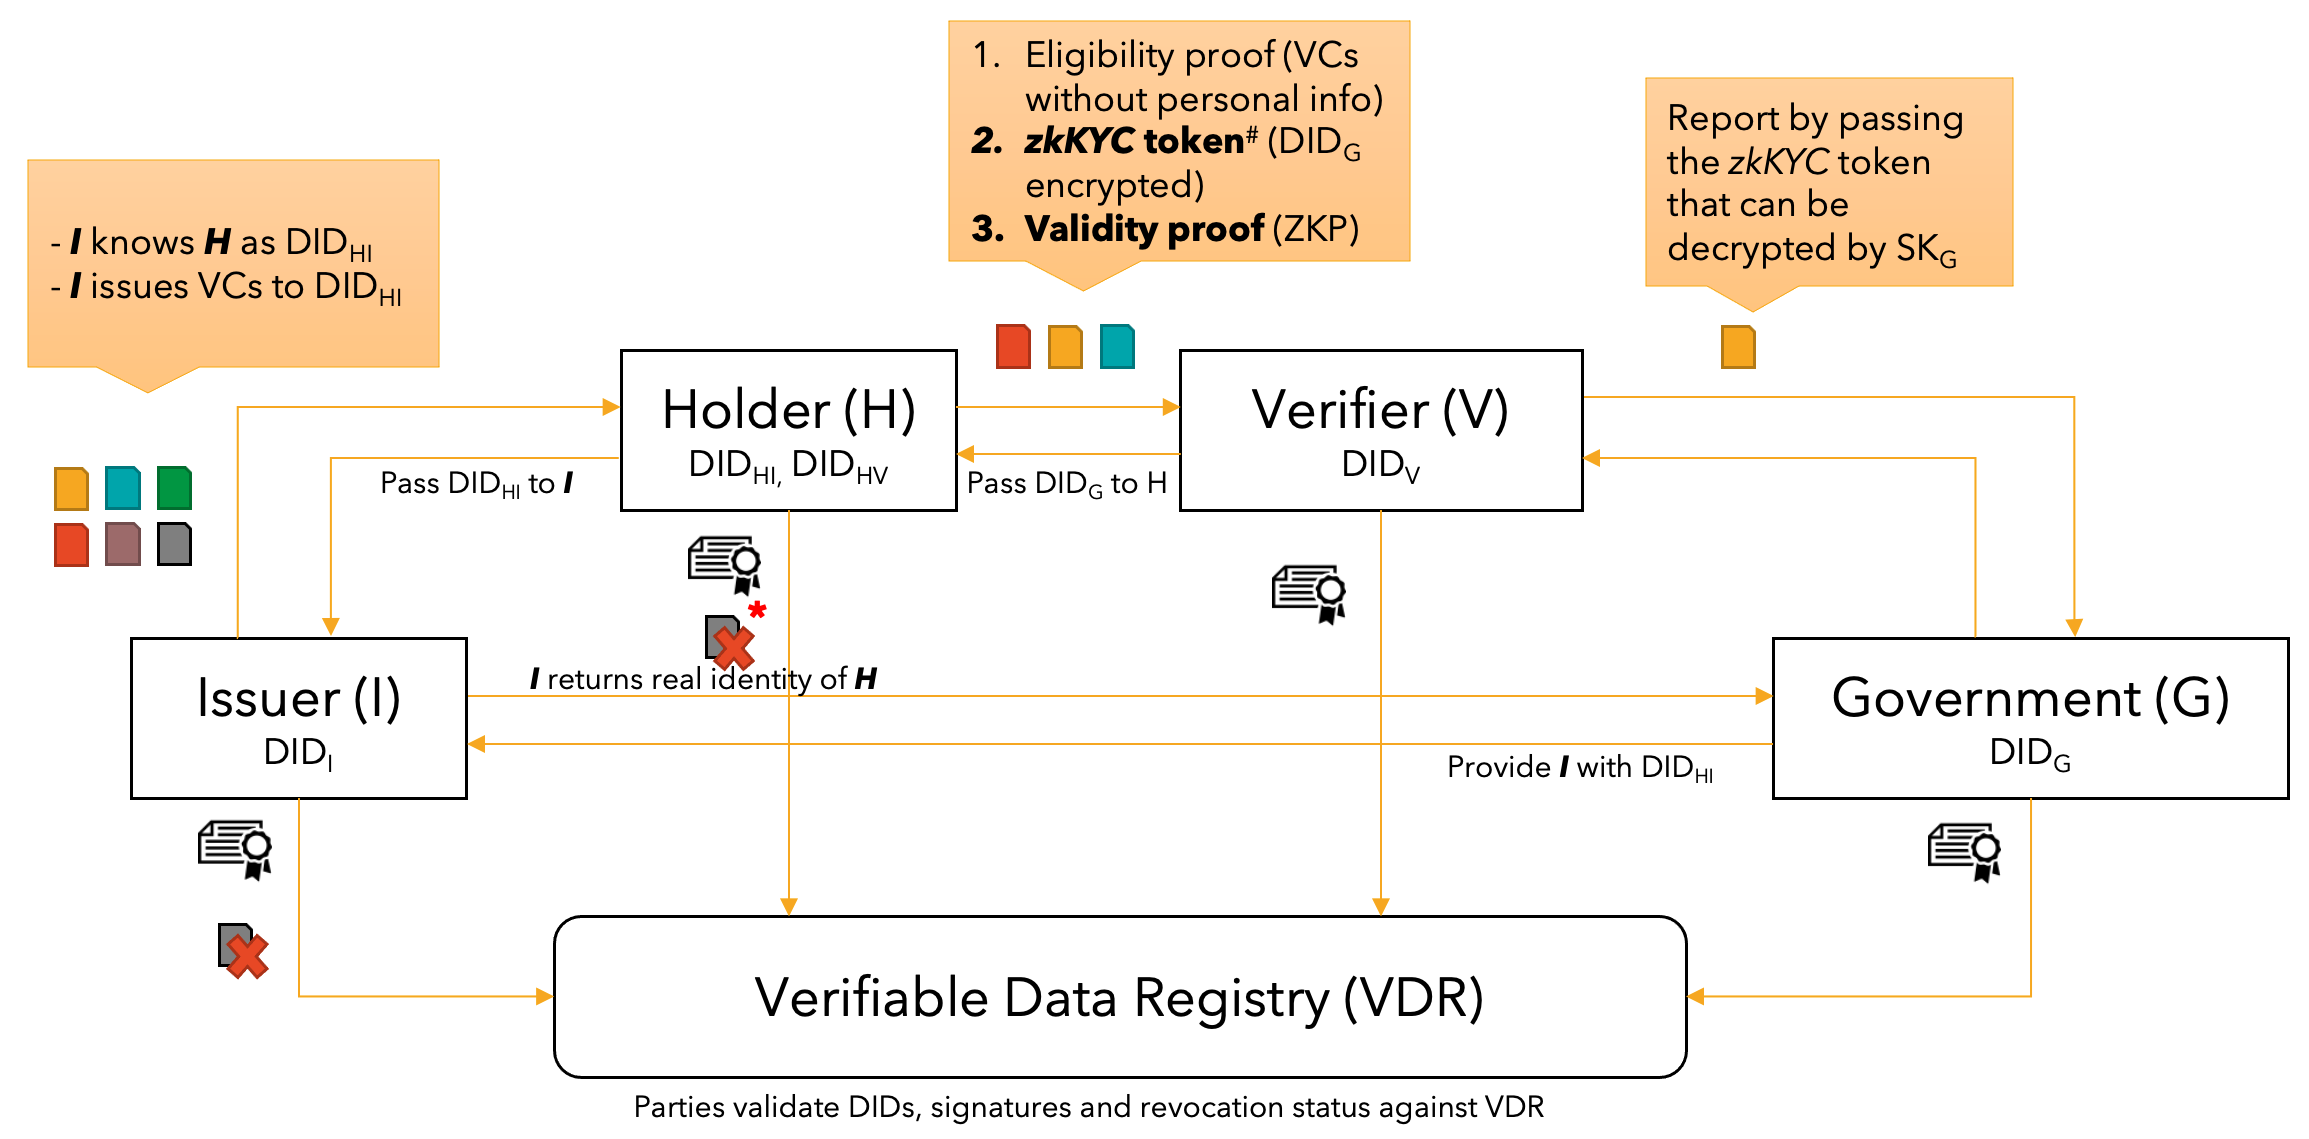
\includegraphics{zkkyc-system.png}
\caption{zkKYC Solution Concept}
\end{figure}

The above figure describes the zkKYC solution concept, where the Issuer
issues credentials to the Holder, which the Holder can use to generate
presentations of eligibility and identity (zkKYC token) for the Verifier.
The Verifier can verify the validity of the information by checking with
the information in the Verifiable Data Registry, which we will discuss
in detail in the next chapter.

The zkKYC token is generated by the user and contains their identity
information, using a zero-knowledge proof system that we designed in
this project. The user can then share the zkKYC token with the business
(verifier) during the KYC process using the SSI system. The business can
then verify the validity of the zkKYC token without revealing any of the
information contained in the token. Only the Government can decrypt the
token to obtain the user's identity under necessary circumstances.

To summarize the roles involved in the zkKYC solution, we have the
following:
\begin{itemize}
\tightlist
\item
\textbf{Issuer:} The Issuer is the entity that controls the real
identity of the user. The Issuer issues the Holder with verifiable 
credentials according to the Holder's information in its database.
In reality, this role can be played by the government agency, or some
large banks that already have the user's information registered via
traditional KYC process.

\item
\textbf{Holder:} The Holder is the user who holds the verifiable
credentials from the Issuer, and may want to register with a new
business, or Verifier. The Holder can generate a zkKYC token using the
verifiable credentials and share it with the Verifier.

\item
\textbf{Verifier:} The Verifier is the business that wants to verify
the identity of the Holder. The Verifier can check the eligibility
of the Holder via the credentials, and verify the validity of the
zkKYC token without revealing any of the information contained in the
token.

\item
\textbf{Government:} The Government is the regulatory authority that
can decrypt the zkKYC token to obtain information to retrieve the
Holder's real identity under necessary circumstances.
\end{itemize}

\subsection*{Business Requirements}

Here are the detailed business requirements of the privacy-preserving KYC
system specified in the original zkKYC paper:

\begin{myquote}
\begin{longtable}[]{@{}
  >{\raggedright\arraybackslash}p{(\columnwidth - 2\tabcolsep) * \real{0.1667}}
  >{\raggedright\arraybackslash}p{(\columnwidth - 2\tabcolsep) * \real{0.8333}}@{}}
\toprule\noalign{}
\begin{minipage}[b]{\linewidth}\raggedright
ID
\end{minipage} & \begin{minipage}[b]{\linewidth}\raggedright
Business Requirement
\end{minipage} \\
\midrule\noalign{}
\endhead
\bottomrule\noalign{}
\endlastfoot
BR01 & The level of user control, agency and privacy provided and
enabled by the self-sovereign identity model MUST be preserved or
enhanced. See section 3.2 for details. \\
BR02 & A User SHOULD NOT share personal identifiable information
(e.g.~name, address, date of birth) when on-boarding at a Business. \\
BR03 & A User MUST prove they meet the criteria defined by the Business
or relevant regulator(s) to consume the provided service (e.g.~adult,
domestic resident, valid driver license for specific vehicle category,
verified email address). \\
BR04 & A Business that suspects a specific User of fraud, money
laundering or terrorism financing MUST be able to report that User to
Government (e.g.~regulator). \\
BR05 & A Business that wants to file charges against a specific User due
to breach of contract or other dispute MUST be able to report that User
to Government (e.g.~law enforcement). \\
BR06 & Government (e.g.~regulator, law enforcement) MUST be able to
identify a reported User based on the information provided and on the
ground of reasonable suspicion. \\
BR07 & When a Business reports a User to Government, this MUST NOT be
disclosed to the User (i.e.~tipping-off). \\
BR08 & A Business SHOULD NOT hold personal identifiable information on a
User, unless it is provided to them by Government in context of a
reported issue. \\
\end{longtable}
\end{myquote}

We designed our implementation according to these requirements. We will
review our system against these requirements after the relevant
discussions.

Finally, we strongly recommend you to read the original zkKYC paper by
Pauwels (2021) to have a better understanding of this solution.

\section{System Architecture}
Ideally, a self-sovereign identity system is decentralized. That means
there can be multiple organizations acting as each role. All of them
are connected to each other via peer-to-peer credential passing and
a decentralized ledger to store the decentralized identity information.
We will introduce the how SSI works in the next chapter. In this section,
we will focus on the system architecture of a single role of the system,
as shown in the following figure.


\begin{figure}[h]
\centering
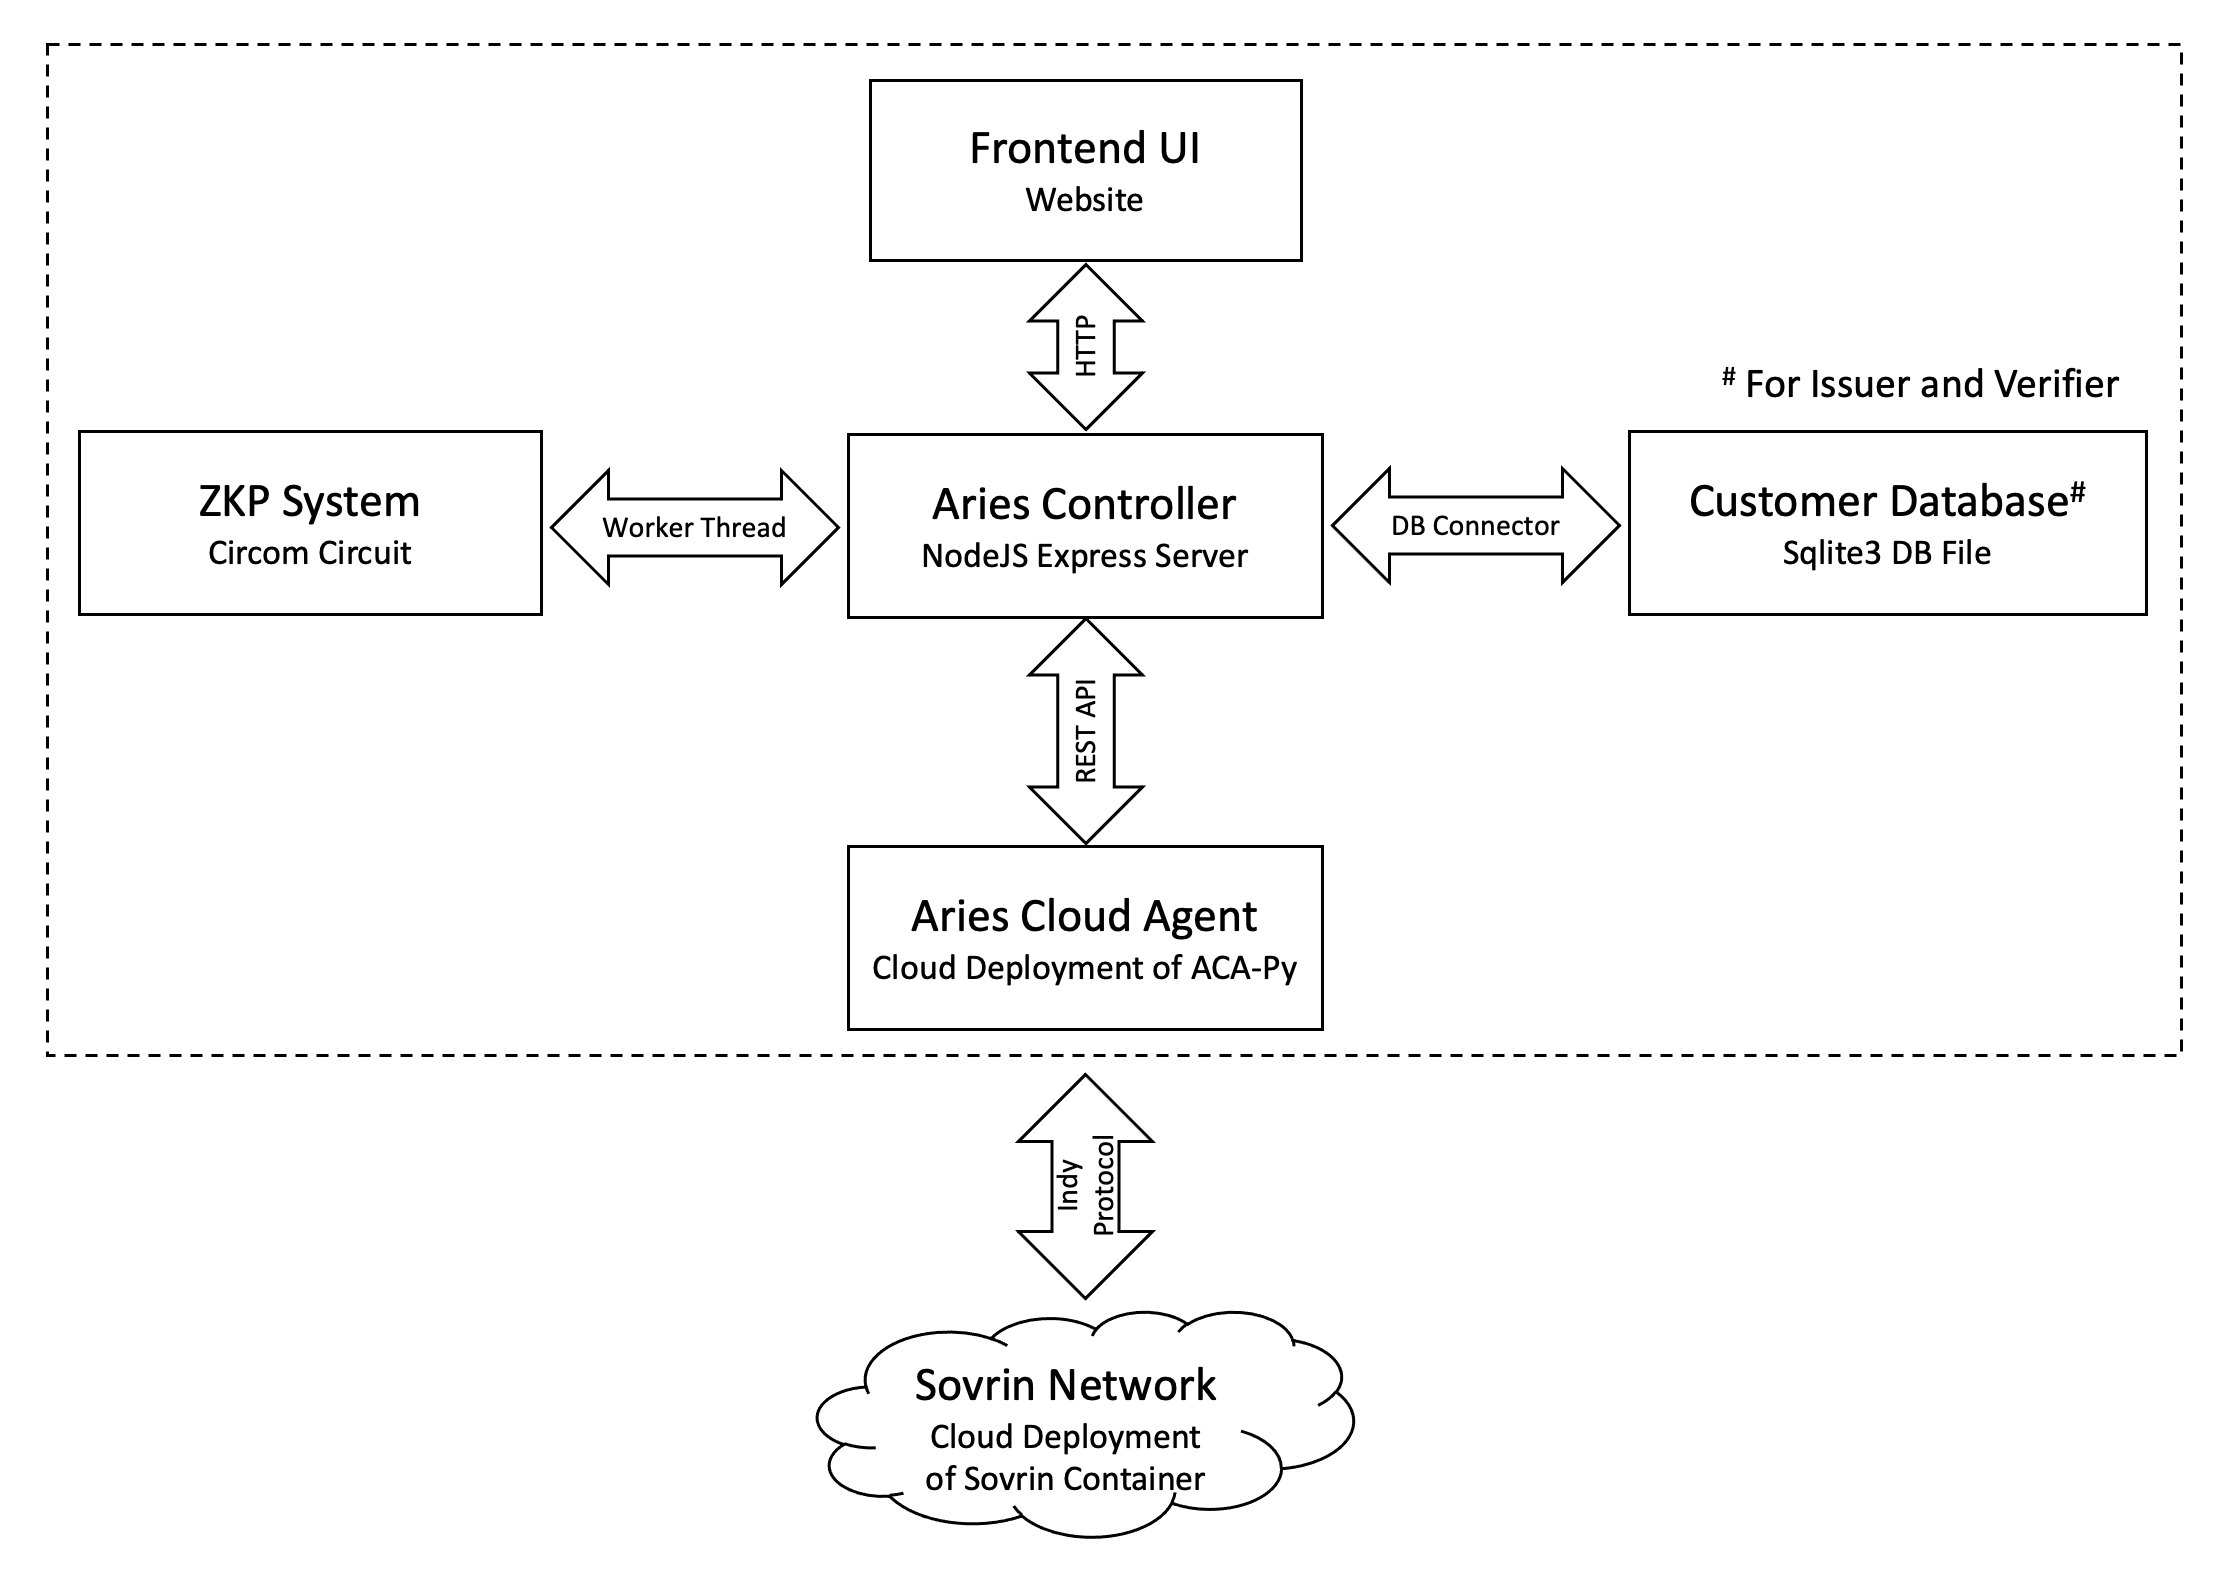
\includegraphics[width=14cm]{sys-arch.png}
\caption{System Architecture for One Role}
\end{figure}

For each role, we have a \emph{frontend UI} for users to interact with. The UI
is connected to the \emph{Hyperledger Aries} controller. The frontend UI
can be a mobile app or a website. In our project, we have implemented
websites as the frontend UI for each role.

The \emph{Aries controller} implements our business logic, such as what to
include in the credential, how to generate the token and proof, what
to do upon receiving a credential and so on. Thus, it is also connected
to the \emph{ZKP system} for zkKYC token generation and verification,
and the \emph{database} for retrieving or storing customers' information.

In our project, we implemented the \emph{Aries controller} using NodeJS.
The \emph{ZKP system} is built using the \emph{zkSNARK} libraries
Circom and SnarkJS. The \emph{database} is simply SQLite3 DB files.

Then, the Aries controller is connected to the \emph{Hyperledger Aries
Framework} via HTTP REST API provided by tha Aries Cloud Agent (ACA-Py).
We have deployed the ACA-Py on a remote server, one for each of the
Issuer, Holder and Verifier. ACA-Py will handle the communication with
the other agents, and perform verification using the information stored
in the distributed ledger of the Sovrin Network, which acts as the
Verifiable Data Registry (VDR) in our system.
\chapter{Self-Sovereign Identity (SSI) Using Hyperledger Aries}

\section{Introduction to SSI}
\subsection{What is Self-Sovereign Identity?}
Self-sovereign identity (SSI) is a term to describe a new approach to
identity administration that allows individuals to control the use of
their personal information. SSI systems are decentralized, meaning that
they do not rely on a central authority to manage identity information.

In traditional identity systems, the identity provider (e.g.~government,
corporation) is responsible for managing the identity information of
individuals. The identity provider is also responsible for verifying
the identity of individuals. In contrast, SSI systems allow individuals
to manage their own identity information and verify their identity
themselves. This is achieved by using cryptographic keys to sign
information and verify the authenticity of the information.

Besides authentication, SSI systems also allow individuals to prove their
eligibility for certain services. For example, an individual can prove
that they are over 18 years old to open an investment account, by
presenting a \emph{verifiable credential (VC)} issued by a trusted
authority and stored in his or her digital wallet. The verifier can
then be assured about the eligibility of the individual without reaching
out to the original issuer, or knowing any unnecessary information.

In this system, the credential issuer decides which attributes to include in
the credential, the holder decides which attributes to disclose to the verifier,
and the verifier decides whether to accept the credential based on the disclosed
information and the credibility of the issuer. The possibility of selective
disclosure of information helps address the \emph{Bundling Problem} as we
discussed in the previous chapter.

\subsection{Key Components in SSI}
Technically, SSI systems are built on top of a set of standards. [ref: w3c-did, w3c-vc]. 
In this sub section, we will discuss the three key components, namely
\emph{Decentralized Identifier (DID)}, \emph{Verifiable Credential (VC)} and
\emph{Verifiable Data Registry (VDR)}.
\subsubsection{Decentralized Identifier (DID)}
The decentralized identifier (DID) is a globally unique identifier the subject.
The subject can be individuals and organizations. The word ``decentralized'' 
also describes the practice that the DID is not managed by a central authority,
but generated by the subject itself.

A DID is a string of characters that consist of three parts: the DID scheme,
the DID method and the method-specific identifier, as illustrated in the
following example:
\begin{figure}[h]
  \includesvg[width=5cm]{parts-of-a-did.svg}
  \centering
\end{figure}
All DIDs start with the string \texttt{did:}. The DID method suggests how the
DID can be resolved to a \emph{DID Document}, such as \texttt{did:ethr} using
the Ethereum blockchain, or \texttt{did:sov} using the Sovrin network.
Each DID method has its own rules for generating and resolving the 
method-specific identifier.

Resolved DID documents are JSON objects that contain the public keys and service
endpoints of the subject. The DID document can be used to verify the authenticity
of the DID and related signatures using the public keys, or to communicate with
the subject using the service endpoints.
\subsubsection{Verifier Credential (VC)}
The Verifiable Credential (VC) is a JSON object that contains a set of attributes
that are relevant to the subject. It is issued by the issuer and stored in the
holder's wallet. The holder can then present the VC to the verifier to prove
their eligibility for certain services. Depending on the DID method, it may be
possible for the issuer to revoke issued VCs.

The credentials are verifiable in the way that the verifier can verify the
validity of the signatures via the public keys in the issuer's DID document,
which is recorded in the \emph{Verifiable Data Registry}.

The signing scheme used in the VC is designed to support selective disclosure,
for example, the CL signature for JSON-LD credentials. Some schemes also 
support predicate proofs, which allow the holder to prove that a certain
attribute is within a certain range, such as age. For example, the BBS+ 
signature.

Finally, with a verifiable credential, the holder can select a subset of its
attributes and generate a VC presentation for the verifier.

\subsubsection{Verifiable Data Registry (VDR)}
A verifiable data registry is where the DID documents, VC schemas and the
revocation list are stored. Ideally, the VDR is a decentralized system that
is not controlled by a single entity. The VDR can be a blockchain, such as
Ethereum, or a distributed ledger, such as Sovrin, which is an instance of
Hyperledger Indy. In our project, we use Sovrin as the VDR.

\subsection{Typical SSI Workflow}

\begin{figure}
\centering
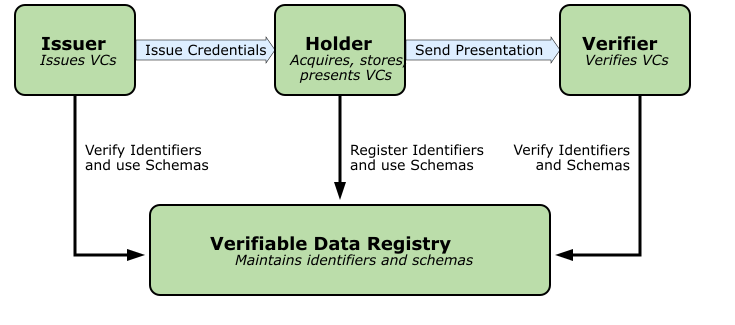
\includegraphics[width=12cm]{ssi.png}
\caption{Typical SSI Workflow}
\end{figure}

\section{Hyperledger SSI Framework}

\subsection{Relevant Hyperledger Projects}
Hyperledger Foundation is a non-profit organization that incubates and
develops open source blockchain projects. In the SSI space, there are three
relevant Hyperledger projects. They are \emph{Hyperledger Aries},
\emph{Hyperledger Indy} and \emph{Hyperledger Ursa}.

The following figure illustrates the relationship between these projects.

\begin{figure}
\centering

\includegraphics[width=8cm]{eco.png}
\caption{Hyperledger SSI Projects}
\end{figure}

The lowest layer is the \emph{Hyperledger Ursa} project, which provides
cryptographic primitives for the other projects. The \emph{Hyperledger
Indy} project provides a distributed ledger for storing DID documents and
VCs. For instance, the Sovrin Network we use in our project is developed
based on the Hyperledger Indy project. The \emph{Hyperledger Aries}
project provides a set of APIs for interacting with the distributed
ledger and communicating with other agents.

\subsection{Hyperledger Aries}
As a developer of SSI applications, we write programs using the Hyperledger
Aries framework. The Aries framework provides a set of APIs that allow
developers to interact with other SSI agents through the underlying SSI
protocols such as \emph{Connection Protocol}, \emph{Credential Exchange
Protocol} and \emph{Present Proof Protocol}. There are also several
implementations of Aries agents, such as \emph{Aries Cloud Agent
Python (ACA-Py)} and \emph{Aries Framework Go}.

In our project, we use ACA-Py as the agent implementation. The following
figure illustrates the architecture of ACA-Py.

\begin{figure}
\centering
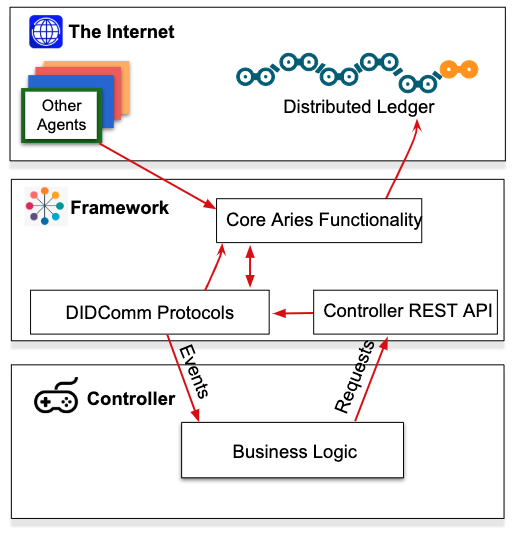
\includegraphics[width=8cm]{aca-py.png}
\caption{Hyperledger Aries Architecture}
\end{figure}

To develop an SSI application with Hyperledger Aries, we need to
implement our business logic in the \emph{controller} of the agent.  
From there, we define which credentials to issue, which attributes to
disclose and which credentials to accept, and so on. With ACA-Py, we
can implement the controller in any programming language and interact
with the framework through the REST API.

\section{Implementing zkKYC with Hyperledger Aries}

In our project, we have four roles, namely \emph{Issuer}, \emph{Holder},
\emph{Verifier} and \emph{Government}. We have implemented agent controllers
for Issuer, Holder and Verifier to demonstrate the SSI workflow of the
zkKYC system for issuing and verifying the credentials of eligibility and
zkKYC token.

The Government may also have its own agent controller of
an SSI agent to communicate with the Issuer and Verifier. For simplicity,
we did not implement the Government agent because what matters from the
Government is just its key pair for encrypting and decrypting the
\emph{zkKYC token}, which we will demonstrate by direct inputs during
encryption and decryption.

\subsection{Environment Setup}
\subsubsection{Hyperledger Aries Cloud Agent}
In our project we use the \emph{Hyperledger Aries Cloud Agent (ACA-Py)}
as the SSI agent. We have deployed the three ACA-Py agents on the same
machine with different ports. The Issuer agent is running on port 8020,
the Holder agent is running on port 8030, and the Verifier agent is
running on port 8040.

For demonstration purpose, we let the each agent connect to an in-memory
Indy wallet. The wallet is a secure storage for the agent's keys,
credentials and information of established connections. The wallet is
encrypted with a master key, which is generated by and managed by the
agent.

\subsubsection{Sovrin Network}
\emph{Sovrin} is a distributed ledger for identity built on top of
Hyperledger Indy. It is a permissioned network, which means that only
authorized entities can join the network. In our project, we deployed a
local Sovrin network using a container running four validator nodes.
Then, we can register new DIDs to our local Sovrin network for development
and demonstration.

\subsection{Major Components}
In this subsection, we will introduce major components of the roles
in our project. For each component, we will start from the frontend user
interface to describe the operations that the user can perform, and then
for each operation, we will describe the corresponding agent controller's
work in the back-end.
\subsubsection{Issuer Site}
The Issuer Site simulates the process of customer real identity registration
with the Issuer, and the process of verifiable credential request and 
issuance. 

First, the customer (holder) need to fill in the registration form and create a
profile with the Issuer. This step demonstrate the traditional KYC process
performed by the Issuer, before it can issue verifiable credentials to the
customer. The customer's profile is stored in the Issuer's database.

Then, before requesting verifiable credentials, the customer needs to setup a 
connection between the Issuer and his/her wallet agent. To do this, he/she
needs to login the Issuer's customer portal and get an invitation URL from
the Issuer. Then, the customer paste this URL into the Holder's Wallet agent.
The Holder's Wallet agent will then setup a connection with the Issuer's
agent in the backend.

During the connection setup, the Holder's agent will generate a dedicated DID,
\texttt{$DID_{HI}$}, for the connection. The issuer will then bind this DID
with the customer's real identity in its database.
Then, the holder can login the Issuer's customer portal to request verifiable
credentials for eligibility proof or \emph{zkKYC}.

The eligibility proof VC contains the customer's personal information such as
age and nationality, which may be required by the verifier. When it is
requested, the Issuer will issue a VC with the customer's personal information
and send it via the connection with the holder's wallet agent.

The zkKYC credential is a special credential we designed in this project for
the zkKYC system. It contains the Issuer's DID, the Holder's DID 
(\texttt{$DID_{HI}$}), and the Issuer's signature on the tuple of these two
DIDs. This credential will be sent to the Holder in the same way as the other
VC.

\subsubsection{Holder's Wallet}
This is the controller for the Holder's wallet agent.

As mentioned above, the first function of the Holder's wallet agent is to
setup a connection. It can accept an invitation URL from either the Issuer
or the Verifier and setup connections to them.

The second function of the Holder's wallet agent is to accept and store the
verifiable credentials issued by the Issuer. The holder can see a list of
credentials stored in the wallet on the frontend.

When registering a business with the Verifier, the Holder will be required
to present a verifiable credential for eligibility proof. Upon getting the
presentation request, the Holder can select the credential from the wallet
and generate a presentation for the Verifier. The presentation process will
be handled by the Holder's wallet agent.

The generation and presentation of the zkKYC token, however, works
differently from the standard SSI procedures. We need to be aware that
what the Holder presents to the Verifier in this step is not the zkKYC
credential itself, but a \emph{zkKYC token}, containing the information in
the original credential from the Issuer AND information about the connection
with this specific Verifier, along with its \emph{validity proof}.

In fact, this step is achieved by generating the zkKYC token and proof
with the ZKP system, which we will discuss in the next chapter, and then
\emph{issuing} a new verifiable credential to the Verifier. Here, we let
the Holder to issue the credential, because the content is actually
generated by the Holder. Upon receiving this credential, the Verifier
can further verify the validity of the zkKYC token through our ZKP system.

\subsubsection{Verifier Site}
Similar to the Issuer Site, the Verifier Site simulates the process of
business registration, but instead of conducting traditional KYC process,
the verifier simply requests for presentation of verifiable credentials
we discussed above.

As already mentioned in the previous subsections, the Holder needs to
setup a connection, by firstly going to the Verifier's customer portal and
getting an invitation URL. Similarly, the Holder will have a dedicated DID
$DID_{HV}$ for the connection.

The credential requests is also initiated from the customer portal by
clicking on the \emph{Credential Request} button. The Verifier will then
send a credential request to the Holder's wallet agent via the connection,
and automatically complete the process when the Holder's wallet agent in
the backend.

The Verifier can later retrieve the zkKYC token of a certain ${DID_{HV}}$
and report it to the Government when it is required.

\subsubsection{Government's Portal}
The Government's portal is a web application that allows the Government to
decrypt the reported zkKYC tokens to get the information about the Holder.

The information contains the Verifier's DID, the Holder's dedicated DID for
the Verifier, the Holder's dedicated DID for the Issuer and the Issuer's
DID. Then, the Government can check if this token is for the reporting
Verifier (to avoid copying/abusing), and ask the Issuer to retrieve the
Holder's real identity from its database using the Holder's $DID_{HI}$.

\subsection{ZKP Integration}
As mentioned in earlier subsections, the zkKYC token and its validity proof
are generated by the ZKP system, which is the ZKP part of this project.
The ZKP system packaged into a NodeJS module named \textbf{zkkyc-js}. It
provides a set of APIs for Issuer to sign the zkKYC token, for Verifier
to parse and verify the zkKYC token, and for Government to decrypt the
zkKYC token.

We integrate \textbf{zkkyc-js} into the SSI backend by letting the
corresponding agents to call the APIs via a \emph{worker thread} of NodeJS.
The worker thread is a separate thread that can be used to perform
time-consuming tasks without blocking the main thread. This is necessary
because the zero-knowledge proof generation and verification are very
slow in comparison to the other operations in the SSI backend, and thus
we have this implementation to avoid blocking the main thread.

The computation results are passed back to the main thread via callbacks,
and then subsequently passed to database or to the frontend.

\chapter{Zero Knowledge Proof (ZKP) with zk-SNARKs}

Generating the \emph{zkKYC token} and the \emph{validity proof} is an
unaddressed challenge in the zkKYC paper. In this section, we will
discuss our approach to solving this problem using zero knowledge proof
with \emph{zk-SNARKs}.

\section{zk-SNARK Fundamentals}

In this section, we will introduce the fundamentals of zk-SNARKs, and
how we can implement zk-SNARKs in our project.

\subsection{What are zk-SNARKs?}

\emph{zk-SNARKs} stands for \emph{Zero Knowledge Succinct
Non-interactive ARgument of Knowledge}. It is a type of zero knowledge
proof that allows a prover to convince a verifier that a statement is
true, without revealing any information beyond the statement itself. The
statement is usually a mathematical expression, and the prover can prove
that the statement is true by providing a \emph{witness} that satisfies
the statement.

There are many zk-SNARK schemes, or proving systems. To understand how
zk-SNARKs achieve zero knowledge proof, we will use a polynomial-based
proving system as an example to demonstrate the mechanism.
{[}ref:Why and How zk-SNARK Works{]}

\subsubsection{Knowledge as Polynomial}

There is an advantageous property of polynomials. Two non-equal
polynomials of degree at most \(d\) can intersect at no more than \(d\)
points. So, when an \(x\) is randomly chosen from \(N\) numbers, the
probability of choosing an intersecting point is \(\frac{d}{N}\), which
is negligible when \(N\) is significantly larger than \(d\).

Therefore, if the prover responds with a correct evaluation of the
polynomial when given a random position \(x\), it is highly confident
that the prover does know the coefficients of the polynomial.

Thanks to this property, we can express knowledge as coefficients of a
polynomial, and easily prove that we know the coefficients.

\subsubsection{Factorization}

There are usually some constraints on the knowledge (polynomial) that
the prover claims to know. For example, the prover claims that he knows
a polynomial of degree \(d\),

\(p(x) = c_{0}x^{0} + c_{1}x^{1} + \ldots + c_{d}x^{d}\),

and it has roots \(x = 1\ \)and \(x = 2\).

Factorization can help us extract these constraints. In the above
example, because \emph{p(x)} has roots \(x = 1\ \) and \(x = 2\)., we
know that \emph{p(x)} can be factorized into

\(p(x)\  = \ t(x)\ h(x)\)\emph{,}

where \(t(x) = (x - 1)(x - 2)\) and is called the \emph{target
polynomial}, and \(h(x)\) is the quotient of \(p(x)\text{/}t(x)\).

So far, the prover and the verifier can try proving in the following
protocol:

\begin{itemize}
\item
  Verifier chooses a random number \(s\), and computes \(t_{s} = t(s)\).
  Then, Verifier passes \(s\) to Prover
\item
  Prover obtains \(h(x) = \frac{p(x)}{t(x)}\) and computes
  \(p_{s} = p(s)\) and \(h_{s} = h(s)\). Then, Prover passes \(p_{s}\)
  and \(h_{s}\) to Verifier
\item
  Verifier verifies \(p_{s} = t_{s} \cdot h_{s}\)
\end{itemize}

However, the proof is valid only if both Verifier and Prover honestly
follow this protocol. The prover can easily cheat by first choosing an
arbitrary value as \(h_{s}\), and then obtain an \(p_{s}\) by multiply
the arbitrary \(h_{s}\) by \(t_{s}\).

\subsubsection{Homomorphic Encryption}

The flaw of the above protocol is caused by passing a plaintext \(s\)
for polynomial evaluation, allowing dishonest provers to fabricate an
equation. This problem can be solved by homomorphic encryption.

A simple homomorphic encryption is

\(E(x) = g^{x}\ \ \ (mod\ n)\),

where \(g\) is a natural number base, and \(mod\ n\) makes it difficult
to solve \(y = E(x)\) for \(x\), due to the high complexity of the
discrete logarithm problem.

Here are two operations supported by \(E(x)\):

\begin{itemize}
\tightlist
\item
  Addition of two encrypted values \(a\) and \(b\):
\end{itemize}

\begin{quote}
\[g^{a + b} = g^{a} \cdot g^{b} = E(a) \cdot E(b)\]
\end{quote}

\begin{itemize}
\tightlist
\item
  Multiplication of an encrypted value \(a\) by an unencrypted value
  \(m\):
\end{itemize}

\begin{quote}
\[\left( g^{a}m \right) = \left( g^{a} \right)^{m} = \left( E(a) \right)^{m}\]
\end{quote}

Now, we can encrypt the random value \(s\) chosen by Verifier before
passing to Prover. As \(E(x)\) does not support exponential operation
encrypted values, the verifier needs to prepare encrypted values of
\(s^{0},s^{1},\ldots,s^{d}\). The original protocol can be updated as
follows:

\begin{itemize}
\item
  Verifier chooses a random number \(s\), and computes \(t_{s} = t(s)\).
\item
  Verifier computes \(E_{s^{i}} = E\left( s^{i} \right)\) for \(i\) in
  \(0,\ 1,\ \ldots,\ d\) and passes \(E_{s^{i}}\) to Prover
\item
  Prover obtains \(h(x) = \frac{p(x)}{t(x)}\)
\item
  Prover computes
  \(E_{p_{s}} = E\left( p(s) \right) = g^{p(s)} = g^{c_{0}s^{0} + c_{1}s^{1} + \ldots + c_{d}s^{d}}\)
\end{itemize}

\[= \left( g^{s^{0}} \right)^{c_{0}} \cdot \left( g^{s^{1}} \right)^{c_{1}} \cdot \ldots \cdot \left( g^{s^{d}} \right)^{c_{d}} = \prod_{i = 0}^{d}\left( E_{s^{i}} \right)^{c_{i}}\]

\begin{itemize}
\item
  Prover computes \(E_{h_{s}}\) in a similar way
\item
  Prover passes \(E_{p_{s}}\) and \(E_{h_{s}}\) to Verifier
\item
  Verifier verifies
  \(E_{p_{s}} = \left( E_{h_{s}} \right)^{t_{s}}\mathbf{\ \  \Rightarrow \ \ }g^{p(s)} = \left( g^{h(s)} \right)^{t(s)}\mathbf{\ \  \Rightarrow \ \ }p(s) = h(s)\ t(s)\)
\end{itemize}

This updated protocol prevents the prover from getting plaintext \(s\)
and directly computing \(t(s)\). However, this does not completely
eliminate the possibility of cheating. Prover can still fabricate an
equation as follows:

\begin{itemize}
\item
  Compute \(g^{t(s)}\) using \(E_{s^{i}}\)
\item
  Find a random value \(r\), let \(z_{h} = g^{r}\),
  \(z_{p} = \left( g^{t(s)} \right)^{r}\), so that
  \(z_{p} = z_{h}^{t(s)}\)
\item
  Now, \(E_{p_{s}}\) and \(E_{h_{s}}\) can be forged by \(z_{p}\) and
  \(z_{h}\) respectively
\end{itemize}

\subsubsection{Knowledge-of-Exponent Assumption (KEA)}

To address the problem above, we need to enforce the prover to obtain
the values via the polynomials \(p(x)\) and \(h(x)\). Note that after
applying the homomorphic encryption, the coefficients of polynomials are
used to \emph{exponentiate} the encrypted values \(E_{s_{i}}\). That is
why KEA can help.

The problem KEA addresses is described as follows:

Alice has a value \(a\). She needs to pass \(a\) to Bob and asks Bob to
perform an exponentiation \(a^{v}\), where the exponent \(v\) is
\emph{only known by Bob}. How can Alice ensure that Bob has performed
the exponentiation for \(a\) with some \(v\), instead of returning some
other values?

The solution is to prepare a \emph{shifted} value
\(a^{'} = a^{\alpha}\ \ \ mod\ n\), where \(\alpha\) is chosen and only
known by Alice. Then, Alice passes \(a^{'}\) along with \(a\), and asks
Bob to perform the same exponential operation on \(a\), \(a^{'}\) to
obtain \(b\), \(b^{'}\). Finally, Alice checks if

\[b^{\alpha} = \left( a^{v} \right)^{\alpha} = a^{\alpha v} = a^{'v} = b^{'}\]

Since Bob cannot obtain \(\alpha\) except by unfeasible brute-forcing,
the only way for Bob to produce \(\left( b,b^{'} \right)\) that
satisfies the above equation is to perform the exponentiation.

Therefore, in addition to steps in the previous protocol, Verifier will
prepare shifted values \(E_{s^{i}}^{'} = g^{\alpha s^{i}}\) to be passed
to Prover along with \(E_{s^{i}}\), and Prover will return \(E_{p_{s}}\)
and \(E_{p_{s}}^{'}\). Finally, if Verifier checks that if
\(\left( E_{p_{s}} \right)^{\alpha} = E_{p_{s}}^{'}\), it proves that
the prover has correctly performed the homomorphic-encrypted
calculation.

\subsubsection{Achieving Zero-Knowledge}

So far, we have achieved sound and complete proving. But values passed
from Prover to Verifier, \(E_{p_{s}} = g^{p(s)}\),
\(E_{h_{s}} = g^{h(s)}\) and \(E_{p_{s}}^{'} = g^{\alpha p(s)}\)
contains some knowledge about the polynomial \(p(x)\) that can be
extracted by Verifier.

Currently, the verifier verifies that these values satisfy

\[E_{p_{s}} = \left( E_{h_{s}} \right)^{t(s)},\left( E_{p_{s}} \right)^{\alpha} = E_{p_{s}}^{'}\]

It is obvious that if the prover exponentiates \(E_{p_{s}}\),
\(E_{h_{s}}\) and \(E_{p_{s}}^{'}\) to the power \(\delta\), the
equations still hold. So, the simple solution is to select a secret
random \(\delta\), calculate
\(E_{zk - p_{s}} = \left( E_{p_{s}} \right)^{\delta}\),
\(E_{zkh_{s}} = \left( E_{h_{s}} \right)^{\delta}\) and
\(E_{zkp_{s}^{'}} = \left( E_{p_{s}}^{'} \right)^{\delta}\) \((mod\ n)\)
and pass the \(E_{zk}\) values to the verifier.

\begin{center}\rule{0.5\linewidth}{0.5pt}\end{center}

There is a sequence diagram on the next page showing the protocol we discussed
above.

\begin{figure}
\centering
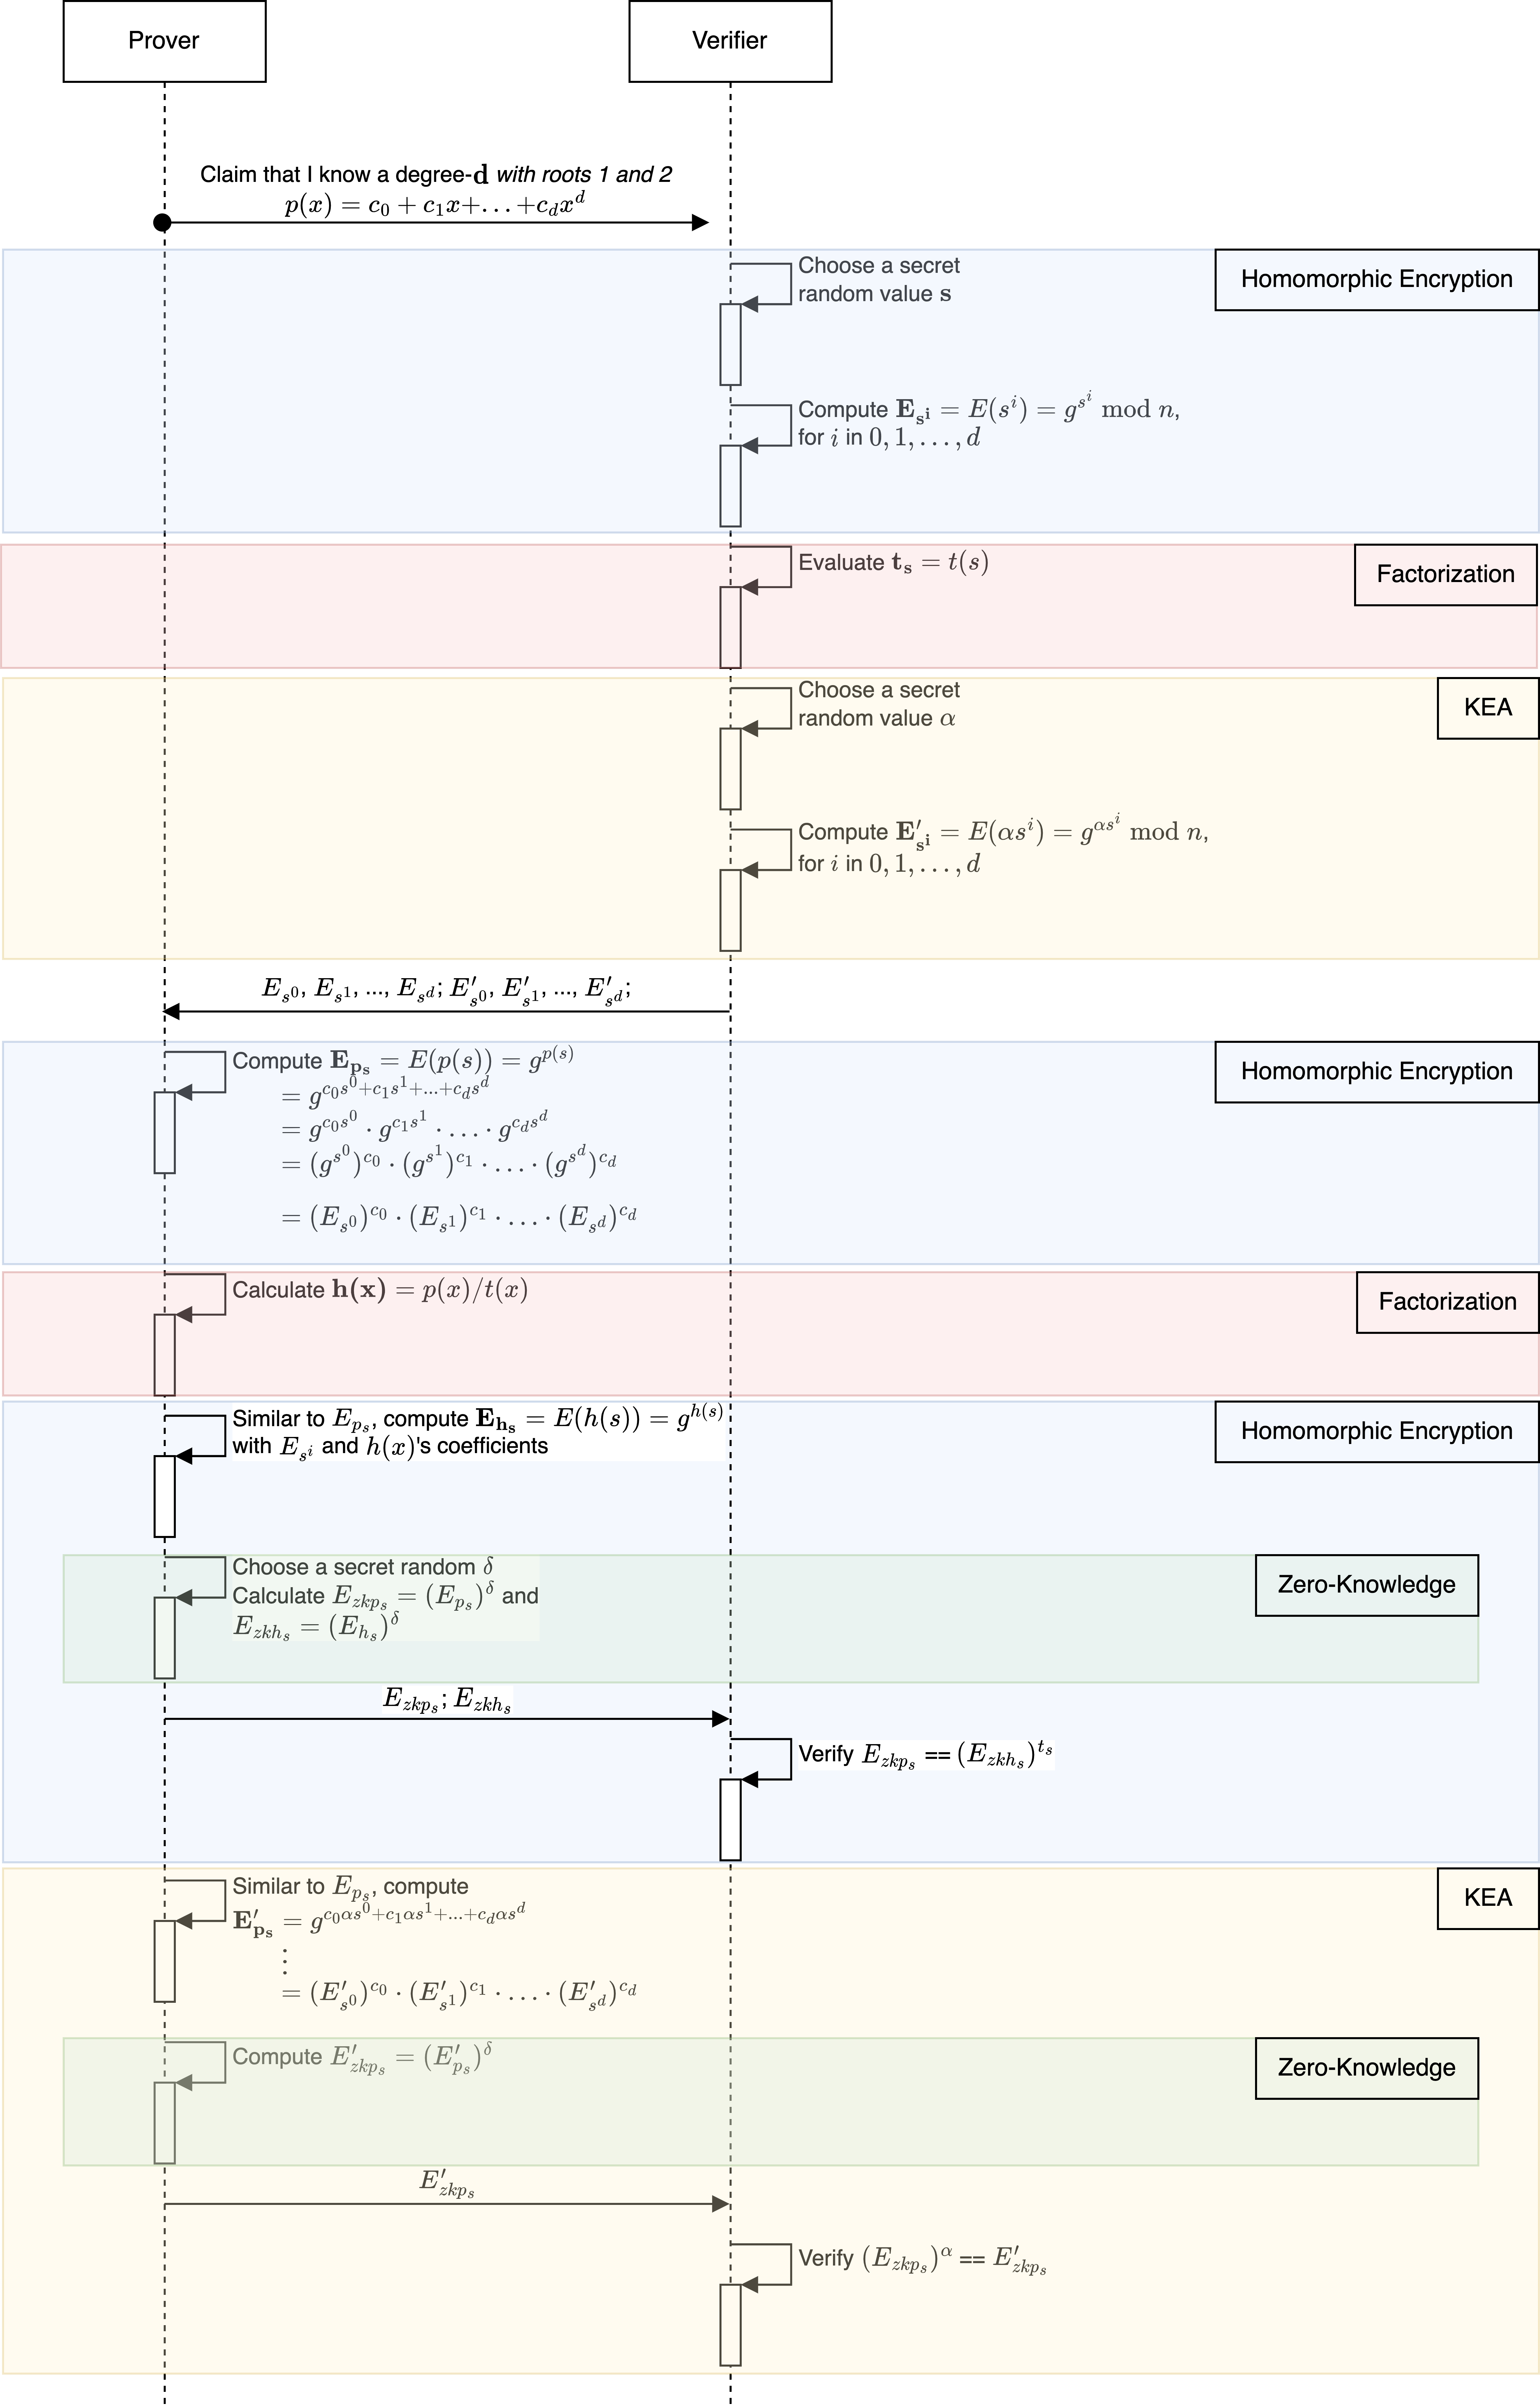
\includegraphics{zksnark.png}
\caption{Sequence Diagram}
\end{figure}

Until now, we have achieved sound and complete zero-knowledge proving.
Full zkSNARK also involves another two properties: succinctness
and non-interactivity, but we will not cover those details in this
report to avoid further distraction from our main topic.

\subsection{Choosing a Proving System}

Groth16 and PLONK are two popular zk-SNARK proving systems.

Groth16 is based on pairing-based cryptography and uses a construction
called \emph{bilinear pairing}. Groth16 is efficient and features
succinct proofs and reasonably fast performance, and it has been widely
adopted in applications such as privacy cryptocurrencies like Zcash.

A major drawback of Groth16 is that it requires a trusted setup for each
different circuit. A trusted setup is a process that generates the
parameters for the proving system. It can be analogous to the process of
generating the encrypted powers of \(s\) to get \(E_{s^{i}}\) in the
previous section.

The trusted setup is a one-time process that is expensive and
time-consuming, and must be performed by trusted parties using secure
Multi-Party Computation (MPC).

PLONK, on the other hand, is a more recently proposed, polynomial-based
zk-SNARK proving system that leverages the \emph{polynomial commitment
scheme}.

The advantage of PLONK is that it supports a universal trusted setup,
which means that the trusted setup can be performed once and used for
any circuit. This is a major improvement over Groth16.

However, PLONK is not as efficient as Groth16 as it has a much slower
performance and larger key and proof sizes. Taking our circuit as an
example, with Groth16, generating the proving and verification keys took
us about 2.5 minutes, and generating the proof took only around 15-20
seconds. The proving key size is 59MB. In contrast, with PLONK, it took
us about 80 minutes to write 407 out 1163 Lagrange polynomials for the
setup, and then the incomplete proving key exhausted all 33GB of free
disk space on our machine\ldots{}

Both Groth16 and PLONK are supported by \emph{SnarkJS}, the tool we will
use to generate the witness and proof. So, either of the two proving
systems may be used in the project. However, due to the prohibitive cost
of PLONK, we will just choose Groth16 in our implementation.

\subsection{Implementing zk-SNARKs in the Project}

To implement zk-SNARKs, we can define zk-SNARK constraints in the form
of a circuit using the \emph{circom language}, and then generate the
witness and proof using \emph{SnarkJS}.

Here are the general steps of the process:

\subsubsection*{A. Circuit definition and preparation for proving}

\begin{enumerate}
\def\labelenumi{\arabic{enumi}.}
\tightlist
\item
  Define the circuit in the circom language.
\item
  Compile the circom file to into a Rank-1 Constraint System (the .r1cs
  file) using the circom compiler. This step also generates the script
  for generating the witness.
\item
  Trusted Setup - Powers of Tau. With Groth16, the first phase, Powers
  of Tau, can be performed in advance. So, we just download the Powers
  of Tau file of the right size from a trusted source
  {[}ref:https://github.com/iden3/snarkjs{]}.
\item
  Trusted Setup - Phase 2. The phase 2 setup, however, is specific to
  the circuit. Ideally, it requires contributions from multiple trusted
  parties via MPC. In our demonstration, we just contribute our
  hardcoded entropy in the phase 2 setup. This step generates the
  proving key (.zkey file) and the verification key
  (verification\_key.json).
\end{enumerate}

\subsubsection*{B. Generating the witness and proof}

\begin{enumerate}
\def\labelenumi{\arabic{enumi}.}
\tightlist
\item
  Prepare the input data for the circuit.
\item
  Generate the witness by executing the witness generation script with
  the correct input data.
\item
  Prove the witness using the proving key, and obtain the proof with
  public inputs and outputs.
\end{enumerate}

\subsubsection*{C. Verifying the proof}

\begin{enumerate}
\def\labelenumi{\arabic{enumi}.}
\tightlist
\item
  Verify the proof, public inputs and outputs using the verification
  key.
\end{enumerate}

\section{ZKP Workflow for zkKYC}

In this section, we will illustrate the zero knowledge proof workflow
using the following scenario:

\begin{itemize}
\tightlist
\item
  Issuer has a public DID \texttt{did\_i} and has a key pair
  (\texttt{pub\_i}, \texttt{priv\_i}).
\item
  Holder generates a peer DID \texttt{did\_hi} to interact with Issuer.
\item
  Verifier has a public DID \texttt{did\_v}.
\item
  Holder generates a peer DID \texttt{did\_hv} to interact with
  Verifier.
\item
  Government has a key pair (\texttt{pub\_g}, \texttt{priv\_g}).
\end{itemize}

Before the zkKYC process, the Holder has already registered with the
Issuer. That is to say, the Issuer has the binding
\texttt{\{\ did:\ "did\_hi",\ real\_name:\ "Evil\ Holder",\ passport\_no:\ "A12345678"\ \}}
in its database.

\textbf{1. Issuer signs the tuple \texttt{(did\_i,\ did\_hi)}.}

When the Holder requests a KYC credential, the Issuer signs the tuple
\texttt{(did\_i,\ did\_hi)} with its private key \texttt{priv\_i}, and
sends the signature \texttt{sig\_i\_hi} to the Holder in the credential.
This conveys that the Holder is a recognized customer of the Issuer.

\textbf{2. Holder generates the zkKYC token and proof for the Verifier.}

When the Holder registers a business with the Verifier, the Holder
generates a zkKYC token and proof for the specific Verifier.

To generate the zkKYC token, the Holder inputs \texttt{did\_i},
\texttt{did\_hi}, \texttt{did\_hv}, \texttt{did\_v},
\texttt{sig\_i\_hi}, \texttt{pub\_i}, \texttt{pub\_g} into the zkKYC
token generation circuit. The circuit will perform the following
steps:

\begin{itemize}
\tightlist
\item
  Verify \texttt{(did\_i,\ did\_hi)} with \texttt{pub\_i} and
  \texttt{sig\_i\_hi}.
\item
  Encrypt \texttt{(did\_i,\ did\_hi,\ did\_hv,\ did\_v)} with
  \texttt{pub\_g} to obtain the \emph{circuit output},
  \texttt{encryptedPayload}.
\item
  Include \texttt{did\_hv}, \texttt{did\_v}, \texttt{pub\_i} and
  \texttt{pub\_g} as \emph{public inputs}.
\end{itemize}

Proof of the execution process is generated with the proving key from
the trusted setup.

Then, the Holder sends public inputs, output and proof to the Verifier.
These can be regarded as the zkKYC token and proof.

\textbf{3. Verifier verifies the zkKYC token and proof.}

When the Verifier receives the information from the Holder, it checks
the following:

\begin{itemize}
\tightlist
\item
  Verify the public inputs and output with the proof using the
  verification key of the circuit, to ensure the enclosed information is
  valid.
\item
  Check the public inputs \texttt{did\_hv} and \texttt{did\_v} to ensure
  that the zkKYC token is intended for the Verifier.
\item
  Check the public input \texttt{pub\_i} to ensure that the Holder is
  registered with a \emph{recognized} Issuer.
\item
  Check the public input \texttt{pub\_g} to ensure that the
  \texttt{encryptedPayload} can be decrypted by the intended Government.
\end{itemize}

With this information, the Verifier cannot deduce any information about
the Holder's identity beyond the Holder's verifier-dedicated DID
\texttt{did\_hv}, but can be assured that the intended party,
Government, can decrypt the information for retrieving the Holder's real
identity.

\textbf{4. Government decrypts the zkKYC token.}

When the Verifier spots suspicious activities of the Holder identified
by \texttt{did\_hv}, the Verifier reports the \texttt{encryptedPayload}
to the Government for further investigation.

Government decrypts the \texttt{encryptedPayload} with its private key
\texttt{priv\_g}, and obtains the tuple
\texttt{(did\_i,\ did\_hi,\ did\_hv,\ did\_v)}. Then, Government can -
check that this is the zkKYC token of the suspicious Holder
\texttt{did\_hv} doing business with the reporting Verifier
\texttt{did\_v}, and - contact the Issuer \texttt{did\_i} to obtain the
Holder's real identity with \texttt{did\_hi}.

Finally, Issuer can retrieve the Holder's real identity,
\texttt{\{\ real\_name:\ "Evil\ Holder",\ passport\_no:\ "A12345678"\ \}},
for the Government to take further actions.

\section{Implementation Details}

Now, we are clear about the workflow of the zkKYC process. In this
section, we will discuss the implementation details of the workflow.
\#\#\# DID Encoding By default, Circom signals are bounded by the field
size of the curve, which is a 254-bit prime number. Therefore, for both
convenience and efficiency, we decide to encode the DIDs in the form of
an array of 248-bit (31-byte) signals. So, DIDs length limits will be
multiples of 31 bytes, and the \emph{multiple} is specified by the
circuit construction parameter \texttt{n248Bits}.

\subsection{Signing and Verification with
EdDSA}

The signing and verification of the tuple \texttt{(did\_i,\ did\_hi)} is
done using EdDSA over the Baby Jubjub curve.

In practice, the signature is created on the \emph{Poseidon Hash} of the
encoded \texttt{did\_i} and \texttt{did\_hi} concatenated together. We
have chosen the Poseidon hash function in favor of the well-known
SHA-256 hash function, because the Poseidon hash function is a set of
permutations over a prime field, which makes it more efficient for
zk-SNARKs.
{[}ref:https://eips.ethereum.org/EIPS/eip-5988{]}

In contrast, the SHA-256 hash function is inefficient in our use case,
and it also resulted in a large number of constraints in the circuits
according to our experiments.

EdDSA Signing is performed in NodeJS using the \_@iden3/js-crypto\_
library, and verification is performed in the circuit using the
\emph{circomlib} library.

The EdDSA signature consists of two elements, \texttt{R} and \texttt{S}.
\texttt{R} is a point on the curve, and \texttt{S} is a scalar. We
encode \texttt{R} as two 254-bit integers in an array, and \texttt{S} as
a 254-bit integer.

In summary, the zkKYC token generation circuit takes the following
inputs for signature verification:

\begin{Shaded}
\begin{Highlighting}[]
\NormalTok{signal input didI[248];  // encoded did\_i}
\NormalTok{signal input didHI[248]; // encoded did\_hi}
\NormalTok{signal input pubI[2];    // public key of Issuer}
\NormalTok{signal input sigS;       // S element of the EdDSA signature}
\NormalTok{signal input sigR[2];    // R element of the EdDSA signature}
\end{Highlighting}
\end{Shaded}

The circuit execution would fail if the signature is invalid.

\subsection{Message Representation in ElGamal Encryption}

Before we discuss the encryption and decryption process, we need to
clarify the message representation in the ElGamal encryption.

Because we implement ElGamal encryption over the Baby Jubjub curve, what
it encrypts is essentially a \emph{point} on the curve. Therefore, we
need a way to represent an arbitrary message with a point on the curve.

An existing solution is to pick a random point on the curve, and
subtract the message from its x-coordinate
{[}ref:https://ethresear.ch/t/elgamal-encryption-decryption-and-rerandomization-with-circom-support/8074{]}
to get a \texttt{xIncrement} value. Then, the message can be represented
by the point and \texttt{xIncrement}.

We improved this solution by performing XOR, instead of subtraction,
between the lowest 253 bits of the x-coordinate and the message up to
253 bits, to get a \texttt{xmXor} value. Note that we do not utilize all
254 bits of the x-coordinate, because otherwise \texttt{xmXor} may
overflow the BabyJub curve field size.

In the existing solution, we need to assert that the x-coordinate of the
point is greater than the message, which can possibly fail, especially
when the message integer is large. In our solution, the encoding can
always succeed.

Also, our solution has the advantage that the representing point, which
acts as the plaintext in the succeeding ElGamal encryption, can be
\emph{uniformly} chosen at random, while the existing solution cannot as
its x-coordinate is lower-bounded by the message. This advantage
increases the security level of the entire encryption process.

\subsection{Token Encryption and Decryption with ElGamal and AES}

This subsection describes how we achieve the public key encryption and
decryption of the zkKYC token.

Encryption is performed in the circom circuit so that we can prove the
proper encryption of the zkKYC token in the zk-SNARK proof, while
decryption is done by the Government in any environment.

Briefly speaking, we first encrypt the payload with AES using a random
symmetric key, and then encrypt the symmetric key with ElGamal using the
Government's public key.

\subsubsection{AES Encryption}

As mentioned in the previous subsection, plaintext messages in ElGamal
encryption are represented by a point and an \texttt{aesKeyXmXor} value.
As the AES key will be later encrypted with ElGamal, it is input to the
circuit as a point \texttt{aesKeyPoint}, and a \emph{public} input value
\texttt{aesKeyXmXor}. Therefore, the first step is to obtain the AES key
by XORing the \texttt{aesKeyXmXor} value with the lowest 253 bits of the
x-coordinate of the point.

The circuit inputs also include the initial vector \texttt{iv} for AES,
which is a randomly generated array of 128 bits.

After obtaining the AES key, we encrypt the payload (\texttt{did\_i},
\texttt{did\_hi}, \texttt{did\_hv}, \texttt{did\_v}) with the key and
\texttt{iv}, into a ciphertext. The \texttt{iv} is then appended to the
ciphertext, and the resulting bit array is the
\texttt{encryptedPayload}.

To encrypt the payload, we use the AES-256-CTR cipher, and the
implementation is adapted from \emph{Electron-Labs/aes-circom}
{[}ref:https://github.com/Electron-Labs/aes-circom{]},
where they implemented the AES-GCM-SIV.

We did not choose AES-GCM-SIV due to its computational complexity, and
we do not require the integrity guarantee it provides. We just use
AES-256-CTR circuit in their repository, and we modified it to match the
bit endianness we are using in the rest of the project.

\subsubsection{ElGamal Encryption}

After AES encryption, we encrypt the AES key with ElGamal using the
Government's public key. With the AES key represented by
\texttt{aesKeyPoint} and \texttt{aesKeyXmXor}, we just apply the ElGamal
encryption on the \texttt{aesKeyPoint}, and output the ElGamal
ciphertext represented by two points \texttt{c1} and \texttt{c2}.

The random number required by ElGamal encryption is taken as an input
signal \texttt{elGamalR}.

In summary, after the encryption process, the circuit takes the
following inputs:

\begin{minted}{c}
signal input didI[n248Bits];  // encoded did_i
signal input didHI[n248Bits]; // encoded did_hi
signal input didHV[n248Bits]; // encoded did_hv
signal input didV[n248Bits];  // encoded did_v
signal input aesKeyPoint[2];  // the point in AES key representation
signal input aesKeyXmXor;     // the xmXor value in AES key representation
signal input aesIV[128];      // the 128-bit AES initial vector
signal input govPubKey[2];    // public key of Government
signal input elGamalR;        // the random number for ElGamal encryption
\end{minted}

and generates the following public information that Government can use
to decrypt the zkKYC token:

\begin{minted}{js}
[
  c1X, c1Y,             // circuit output
  c2X, c2Y,             // circuit output
  ...encryptedPayload,  // circuit output
  aesKeyXmXor           // circuit public input
]
\end{minted}

\subsubsection{Decryption Process}

Using the above public information, the Government can decrypt the zkKYC
token by the following steps:

\begin{itemize}
\tightlist
\item
  Decrypt \texttt{{[}c1X,\ c1Y,\ c2X,\ c2Y{]}} with the Government's
  private key to obtain the AES key point \texttt{aesKeyPoint}.
\item
  XOR the lowest 253 bits of the x-coordinate of \texttt{aesKeyPoint}
  with \texttt{aesKeyXmXor} to obtain the AES key.
\item
  Decrypt \texttt{encryptedPayload} with the AES key to obtain the
  payload (\texttt{did\_i}, \texttt{did\_hi}, \texttt{did\_hv},
  \texttt{did\_v}).
\end{itemize}

\subsection{Bit Lengths of Components --- 248, 253, 254 or 256?}

You may have noticed that we use various bit lengths in the project
implementation. Those values are carefully chosen to maximize the
security of the system, while avoiding overflow. In this subsection, we
will summarize bit lengths for the components and explain the rationale
behind those choices.

Generally, signals in a Circom circuit should be bounded by the finite
field that the underlying elliptic curve is defined on. In our case, the
\emph{Baby Jubjub Elliptic Curve} is defined over the field \(F_p\),
where \(p\) is a \emph{254-bit} prime number
{[}ref:https://eips.ethereum.org/EIPS/eip-2494{]}. Given
this fact, we define the bit lengths for the following components in the
project:

\textbf{DID Representation (248 bits):} A DID is represented by
an array of 248-bit unsigned integers. Each integer can be interpreted
as a 31-byte string.

\textbf{AES Key (253 bits):} We use a 253-bit key for AES-256
encryption, instead of the standard 256-bit key. This is because this
key will be encoded into a point on the Baby Jubjub curve and an XOR
value as discussed in an earlier subsection. Therefore, as the point
coordinate is bounded by a 254-bit number, we need to limit the key size
to 253 bits to avoid overflowing the XOR value.

\textbf{XOR Value (253 bits):} The XOR value, named
\texttt{xmXor}, is used to encode the AES key into a point on the Baby
Jubjub curve. It is the result of XORing the 253-bit AES key with the
lowest 253 bits of the x-coordinate of the encoding point
\texttt{aesKeyPoint}.

\textbf{ElGamal random value \texttt{r} (253 bits):} The random
value \texttt{r} is a signal in the ElGamal encryption circuit. Signals
are bounded by a 254-bit number. When generating the \texttt{r},
however, we use a 253-bit random number to avoid overflowing the signal.

\textbf{Baby Jubjub Point (254 bits):} A point on the Baby Jubjub
curve is represented by two 254-bit unsigned integers or buffers. Public
keys, \texttt{R} in the EdDSA signature, the encoding point
\texttt{aesKeyPoint}, ``shared secret'' \texttt{s} in ElGamal
encryption, and the \texttt{c1} and \texttt{c2} of the ElGamal
ciphertext are all Baby Jubjub points.

\textbf{Private Key (256 bits):} We use a 32-byte buffer as the
private key for the EdDSA signature. Internally, EdDSA derives a 253-bit
scalar from the private key, which is used for the signature generation
process.

\textbf{Private Key Scalar (253 bits):} A 253-bit scalar derived
according to the Baby Jubjub EdDSA signature scheme. It is also used as
the private key for the ElGamal decryption.

\textbf{AES Circuit Input (256 bits):} As the AES-256 algorithm
requires the size of the input to be the multiple of the unsigned
integer size, we pad input units (integers representing DIDs) to 256
bits with trailing zeros. The 253-bit AES key is also padded to 256 bits
with trailing zeros before inputting into the AES circuit.

\subsection{Interfaces and Packaging}

The ZKP part of this project is relatively independent of the SSI part.
So, we group the ZKP actions by roles and define the interfaces as
follows:

\textit{\textbf{Issuer}}
\mint[breaklines]{ts}|generateKeyPair(privKey?: string) => { priv: string, pub: string[] }|
Generate a key pair for the issuer. If \texttt{privKey} is provided,
the key pair will be derived from the private key. Otherwise, a random
private key will be generated.
\mint[breaklines]{ts}|signDidRecord(didI: string, didHI: string, privKey: string) => { s: string, r: string[] }|
Sign the DID record with the private key.

\textit{\textbf{Holder}}
\mint[breaklines]{ts}|generateZkKycProof(didI: string, didHI: string, didHV: string, didV: string, sigS: string, sigR: string[], issuerPubKey: string{[}{]}, govPubKey: string{[}{]}) => { proofJson: string, publicJson: string }|
Generate the zkKYC proof and public information, including the
encrypted contents and public keys.

\textit{\textbf{Verifier}}
\mint[breaklines]{ts}|parsePublic(publicJson: string) => { aesKeyPointCipher: { c1: string[], c2: string[] }, encryptedPayload: string, didHV: string, didV: string, issuerPubKey: string[], govPubKey: string[], aesKeyXmXor: string }|
Parse the public information generated by the Holder into an object.
The parsed object can be easily read by the Verifier and passed to the
government for decryption.
\mint[breaklines]{ts}|verifyZkKycProof(proofJson: string, publicJson: string) => boolean|
Verify the zkKYC proof and public information to check if the information is valid.

\textit{\textbf{Government}}
\mint[breaklines]{ts}|decryptToken(parsedPublic: string, privKey: string) => { didI: string, didHI: string, didHV: string, didV: string }|
Decrypt the zkKYC token with the Government's private key to obtain
the DIDs in the token.

\mint[breaklines]{ts}|generateKeyPair(privKey?: string) => { priv: string, pub: string[] }|
Generate a key pair for the issuer. If \texttt{privKey} is provided,
the key pair will be derived from the private key. Otherwise, a random
private key will be generated.

These interfaces are packaged into a NodeJS module \textbf{zkkyc-js} and
can be imported into the SSI controller written in NodeJS. For this
method, we strongly suggest using separate \emph{worker threads} to run
the zkKYC actions to avoid blocking other tasks in the SSI controller
thread, because the ZKP process is very time-consuming and NodeJS is
single-threaded.

We also implemented GRPC services for these interfaces to facilitate the
integration with SSI controllers written in other languages. You can
start the GRPC server by running \texttt{npm\ run\ grpc} in the
\textbf{zkkyc-js} directory.

\chapter{Project Review}
\section{Business Requirements Review}
This section provides a review of how the business requirements mentioned
in the \hyperref[solutionoverview]{Solution Overview} are met by the zkKYC solution.
\begin{longtable}[]{@{}
  >{\raggedright\arraybackslash}p{(\columnwidth - 2\tabcolsep) * \real{0.1667}}
  >{\raggedright\arraybackslash}p{(\columnwidth - 2\tabcolsep) * \real{0.8333}}@{}}
\toprule\noalign{}
\begin{minipage}[b]{\linewidth}\raggedright
Requirement ID
\end{minipage} & \begin{minipage}[b]{\linewidth}\raggedright
Approach to Meet the Requirement
\end{minipage} \\
\midrule\noalign{}
\endhead
\bottomrule\noalign{}
\endlastfoot
BR01 & We are just added the \emph{zkKYC} token generation and verification
process to the existing SSI solution. Therefore, all properties provided
by SSI is preserved. \\
BR02 & 1. The personal identifiable information is stored in the Issuer's
database. What is shared with the business (Verifier) is an encrypted
token containing the information for the Issuer to retrieve the
information of the given customer. Therefore, the user does not need
to share personal identifiable for KYC with the Verifier. There is also
no way for the Verifier to retrieve the customer's information from the
Issuer as the necessary information for doing so can only be decrypted
by the Government. \\
BR03 & This can be achieved by existing SSI solution with the
verifiable credentials. Aries Framework can handle signing and
verifying such credentials. \\
BR04 & The business (Verifier) can report the zkKYC token to the
Government. The Government can decrypt the token with its private key
and take further actions. \\
BR05 & Same as BR04. \\
BR06 & The Government can decrypt the zkKYC token with its private key
and get the Holder's DID registered in Issuer's database. Then, it can
retrieve the Holder's real identity from the Issuer specified by the
Issuer DID, which is also in the zkKYC token. \\
BR07 & The zkKYC token is stored in the Verifier's secure storage and
can be directly passed to the Government without notifying the
Holder. \\
BR08 & What the business holds is just an encrypted token dedicated to
this business. Only the Government can decrypt the token. \\
\end{longtable}
\section{Security Review}
In this section, we will discuss how our implementation of the zkKYC
solution can protect users' privacy against the following threats:

\textbf{Signature Correlation} ~ Signature correlation means that
different Verifiers may collude to correlate the Holder's identity
via identical signatures from the same Issuer for the Holder. This
is prevented in our solution, because the signature verification is
performed by the ZKP system in the circuit. The Verifiers will not
get the signatures from the Issuer, but just a ZKP proof that the
information is signed by the Issuer controlling a given public key.

\textbf{Verifier Abusing KYC Data} ~ In traditional KYC, the Verifier
may be able to abuse the information provided for KYC purpose. However,
in our system, the Verifier only gets an encrypted token, without any
personal information of the customer. The token is generated by the
Holder specifically for this business. Therefore, it is also meaningless
for other businesses.

\textbf{Holder's Credentials Stolen} ~ If someone steals the Holder's
credentials, they may be able to impersonate the Holder to generate
zkKYC tokens for other businesses. Firstly, the credentials are stored
in the Holder's secure storage of the wallet, which should be generally
safe. Secondly, in case the attacker gets the access to the Holder's
wallet, the Holder can contact the Issuer to revoke the credentials.

\textbf{Data Leakage} ~ In traditional KYC, the Holder's personal
information is stored in the every business they have conducted KYC
with, and thus leads to significant risk of data leakage. If one of
the business is compromised, the user's data is threatened. In our
solution, businesses do not store user's personal data, and the KYC
information is only meaningful for the dedicated businesses.
Therefore, as long as the Issuer is secure, the Holder's data is safe.
This significantly reduces the risk of data leakage threatening the
user privacy.

\section{Limitations}

\begin{itemize}
\tightlist
\item
For the sake of simplicity, we did not implement a full-fledged SSI
system, because our focus is to demonstrate the possibility of
integrating the zkKYC idea into an existing SSI system. In reality,
we can find many more completed SSI solutions.
\item
The payload of the zkKYC token is limited to a small size. Limited by
the efficiency of the proving system, we can only encrypt a small
amount of data in the zkKYC token. In our project, the limit is
four 31-byte DIDs, 124 bytes in total, and that will already take
around 15 seconds to generate the zkKYC token.
\item
The zero-knowledge proof requires us to perform trusted setup by
ourselves. Ideally, this should be performed by a group of reputable
parties. Therefore, it may be difficult to apply the zkKYC solution
with the current proving system in practice and get trusted by the
public.
\end{itemize}

\chapter{Future Work}

\textbf{Optimize Implementation} ~ For simplicity, we did not consider
the performance and efficiency of the implementation in this project. We
can identify several areas for optimization:

\begin{itemize}
\tightlist
\item
  Compared to ElGamal encryption, ECDH is more efficient and secure. We
  can use ECDH to derive the shared secret for symmetrically encrypting
  the DIDs payload.
\item
  AES-256 encryption results in large circuits. For instance, our
  circuit uses the plain AES-256-CTR circuit to encrypt just 32 bytes of
  data, but has more than 120,000 constraints and generates a 21.7MB
  R1CS file! We should find some \emph{zk-friendly} alternatives for
  token symmetric encryption.
\item
  For clearer demonstrations, we used the uncompressed form of Baby
  Jubjub points in the project (two 254-bit integers). In practice, we
  can pack a point into one single 255-bit integer to improve
  efficiency.
\end{itemize}

\textbf{Adapt to a Common Elliptic Curve} ~ We use the Baby Jubjub curve
in this project, which is a special curve designed for zkSNARKs and the
only reliable curve available at the moment. However, it is not widely
used in practice. We may want to consider adapting the project to a more
common elliptic curve, such as the Ed25519 curve. As a prerequisite,
this will need an \emph{efficient} circom implementation of the curve.

\textbf{Explore Other Proving Systems} ~ We use the Groth16 proving
system in this project. However, we may want to consider other proving
systems in practice, because Groth16 requires a trusted setup for each
circuit, and this may not always be practical. Further study and
research are needed to find the most suitable proving system for zkKYC.

\textbf{Integrate into DeFi Protocols} ~ This could be the most exciting
potential of the project, and has also been discussed in the succeeding
zkKYC paper -- \emph{zkKYC in DeFi}
{[}ref:https://eprint.iacr.org/2022/321{]}. This project
can be easily extended to integrate with DeFi protocols, as Circom can
generate Solidity smart contracts for proof verification. Then, a DeFi
protocol can include the zkKYC verification process in its smart
contract, and require users to submit a valid zkKYC proof before they
can use the protocol. This will enable DeFi protocols to provide a more
trustful and still privacy-preserving service to authenticated users.

\chapter{Conclusion}

In this project, we have implemented a zkKYC solution concept based on
the zkKYC paper
{[}ref:https://eprint.iacr.org/2020/1186{]} and the
zkSNARKs technology. We have also integrated the zkKYC solution into the
SSI controller written in NodeJS, and demonstrated the zkKYC process in
a simple use case. .. contribution \ldots{}

\chapter{References}

\end{document}
